%%=============================================================================
%% Methodologie
%%=============================================================================

\chapter{\IfLanguageName{dutch}{Methodologie}{Methodology}}%
\label{ch:methodologie}

%% TODO: In dit hoofstuk geef je een korte toelichting over hoe je te werk bent
%% gegaan. Verdeel je onderzoek in grote fasen, en licht in elke fase toe wat
%% de doelstelling was, welke deliverables daar uit gekomen zijn, en welke
%% onderzoeksmethoden je daarbij toegepast hebt. Verantwoord waarom je
%% op deze manier te werk gegaan bent.
%% 
%% Voorbeelden van zulke fasen zijn: literatuurstudie, opstellen van een
%% requirements-analyse, opstellen long-list (bij vergelijkende studie),
%% selectie van geschikte tools (bij vergelijkende studie, "short-list"),
%% opzetten testopstelling/PoC, uitvoeren testen en verzamelen
%% van resultaten, analyse van resultaten, ...
%%
%% !!!!! LET OP !!!!!
%%
%% Het is uitdrukkelijk NIET de bedoeling dat je het grootste deel van de corpus
%% van je bachelorproef in dit hoofstuk verwerkt! Dit hoofdstuk is eerder een
%% kort overzicht van je plan van aanpak.
%%
%% Maak voor elke fase (behalve het literatuuronderzoek) een NIEUW HOOFDSTUK aan
%% en geef het een gepaste titel.

\section{Gantt diagram}
In figuur ~\ref{fig:methodologie2} is een Gantt diagram te zien van de methodologie. Hierin is te zien hoeveel tijd er aan elke fase wordt besteed en wanneer deze fases zullen plaatsvinden.
\begin{figure}[h]
    \centering
    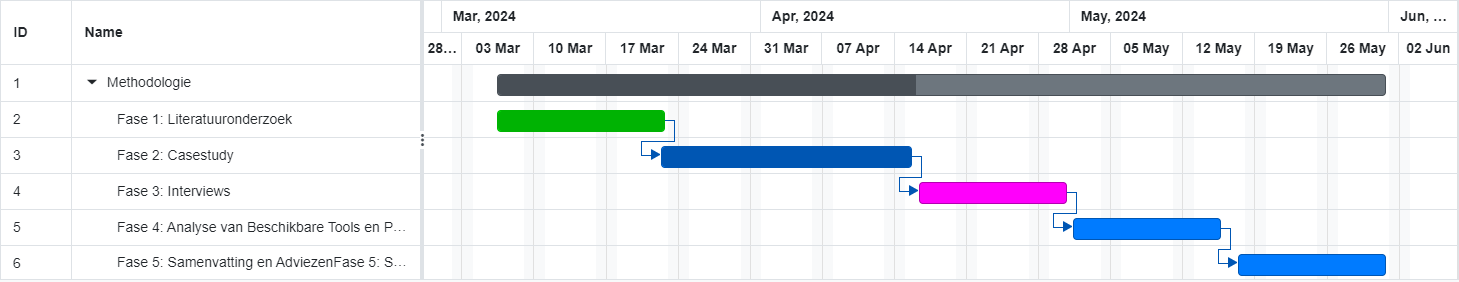
\includegraphics[width=\textwidth]{methodologie2.png}
    \caption{Schematische weergave van de methodologie}
     \label{fig:methodologie2}
\end{figure}
\newpage

\section{Fase 1: Literatuuronderzoek}
Fase 1 omvat een grondige literatuurstudie om de huidige staat van ERP-patchmanagement bij managed service provider te doorgronden. In dit kader worden relevante bronnen ontleed, waaronder 
academische publicaties en vakliteratuur. De kern ligt op het verdiepen van het begrip binnen patchmanagement, het opsporen van bestaande procedures voor patchmanagement en de erkenning van de uitdagingen en succescomponenten. Aan deze fase wordt de volledige tijdsduur van deze bachelorproef besteed.
\section{Fase 2: Casestudy}
De tweede fase omvat het uitdiepen van een specifiek geval door middel van een casestudy bij een managed service provider. De analyse zal zich richten op hoe de onderneming het patchmanagementproces beheert. Dit
proces zal schematisch in kaart worden gebracht aan de hand van een BPMN-schema. De verwachte tijdsbestek voor deze fase is vier weken.
\section{Fase 3: Interviews}
Fase 3 is bedoeld om een gedetailleerder inzicht te verwerven in de tactieken van een managed service provider in relatie tot ERP-patchmanagement. Hiertoe zullen interviews plaatsvinden met bijvoorbeeld ERP-expertisehouders. Deze 
interviews proberen te achterhalen hoe de geïnterviewde naar het proces uit Fase 2 kijkt en waar volgens de geïnterviewde verbeteringen kunnen worden doorgevoerd. De geplande duur voor deze fase is drie weken.
\section{Fase 4: Analyse van Beschikbare Tools en Praktijken}
In de vierde worden praktijken en technologieën voor ERP-patchmanagement geanalyseerd. In deze fase staan we stil bij hoe we het proces voor patchmanagement kunnen verbeteren met behulp van tools en praktijken met. De verwachte periode voor deze fase is drie weken.
\section{Fase 5: Samenvatting en Adviezen}
In de slotfase worden de resultaten van het literatuuronderzoek, de analyses, gesprekken en het casusonderzoek samengebracht. Uit deze synthese worden conclusies getrokken en specifieke adviezen geformuleerd om de effectiviteit 
van ERP-patchmanagement in organisaties te verbeteren. Het tijdsbestek voor deze fase is twee weken. \\


